\section{Task 2 - Questions on dual solution}

\textbf{
    (a) For each scenario, extract the shadow variable to the nodal energy balances and weight it by the nodal demand in the north and south, respectively. What do they represent? Why are they different in the two regions? When do you observe the highest values and why? (0.5)
    }

The nodal electricity price at each node $n$ and time step $t$ is derived from the dual variable $\mu_n(t)$ of the power balance constraint, divided by the time resolution $\Delta t = 3\,\text{h}$:

\begin{equation*}
    \lambda_n(t) = \frac{\mu_n(t)}{\Delta t} \qquad \left[\frac{\text{EUR}}{\text{MWh}}\right]
\end{equation*}

The demand-weighted average price for each region is then computed as:

\begin{equation*}
    \bar{\lambda}_n = \frac{\displaystyle\sum_t \lambda_n(t)\cdot d_n(t)}{\displaystyle\sum_t d_n(t)}
\end{equation*}

\autoref{fig:2a_prices} shows the sorted nodal price duration curves for both scenarios and both regions.

\begin{figure}[!htbp]
    \centering
    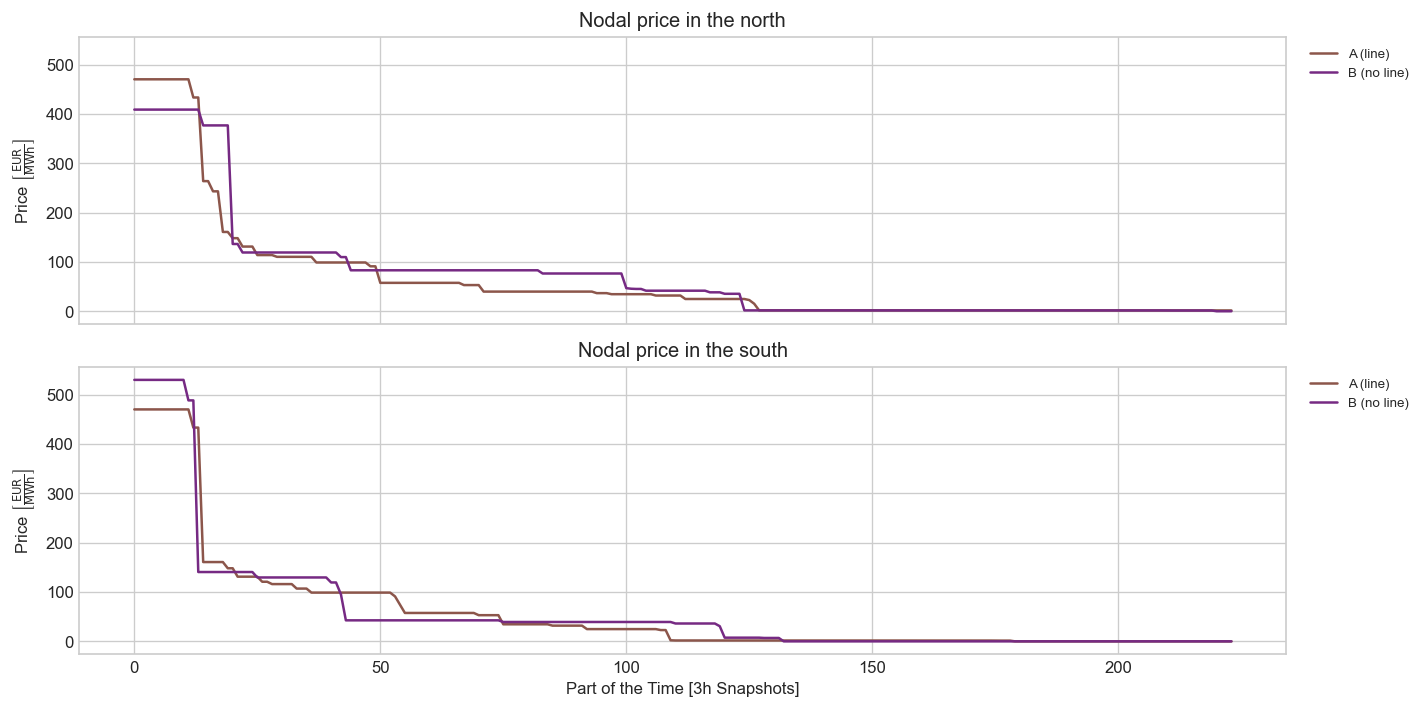
\includegraphics[width=1\linewidth]{Images/fig_2a_prices.png}
    \caption{Nodal price duration curves for scenarios A (line) and B (no line) in each region.}
    \label{fig:2a_prices}
\end{figure}

The price duration curve shows the nodal price for each share of the time, sorted from high to low.
For example, in roughly the most expensive fifth of the hours the price is above $100\,\frac{\text{EUR}}{\text{MWh}}$. 
The dual variable of the nodal energy balance represents the marginal cost of supplying one additional MWh at the respective node, i.e.\ the local electricity price ($\frac{\text{EUR}}{\text{MWh}}$).
Weighting it by the nodal demand gives the average price paid by consumers in that region over the modelled period. \\
In scenario B, prices differ because each node forms its own price independently. The south has large near-zero-cost midday solar surpluses that pull its average down, while the north's wind-dominated mix has almost no surplus hours, so wind's variable cost ($1.62\,\frac{\text{EUR}}{\text{MWh}}$) sets the price most of the time, resulting in a higher average. In scenario A, the line couples the two prices during hours of full capacity, flattening both duration curves and bringing regional averages closer together. \\
The highest price values are observed during dark-lull hours when neither wind nor solar generation is available.
In these scarcity periods the only remaining dispatchable source is the H\textsubscript{2} fuel cell, whose dispatch sets the marginal price. In scenario B the extreme price peaks occur in the south, as a solar-only region it is most exposed when there is no sunshine.
In scenario A the transmission line couples both nodes during scarcity, so both regions reach the same peak price simultaneously (the southern extreme is lowered and the northern peak is raised until they converge).

\textbf{
    (b) In the transmission scenario, consumers of which region benefit more from the transmission line: the north, the south, or both equally? Briefly explain. (0.5)
    }

\autoref{fig:2b_prices} compares the demand-weighted average nodal prices for both regions across the two scenarios.



Consumers in the north benefit more from the transmission line, although both regions gain.
Northern consumers benefit more. In scenario B the north had the higher average price due to its tight wind-solar mix with almost no zero-price hours. The line gives the north access to cheap southern solar surplus, avoiding additional PV and storage investment and producing a larger absolute price reduction. The south benefits too, as it can export surplus instead of curtailing it and needs less storage, but its price reduction is smaller.

The line thus balances the two nodal prices and reduces them in both regions, but to a greater extent in the north.

\begin{figure}[H]
    \centering
    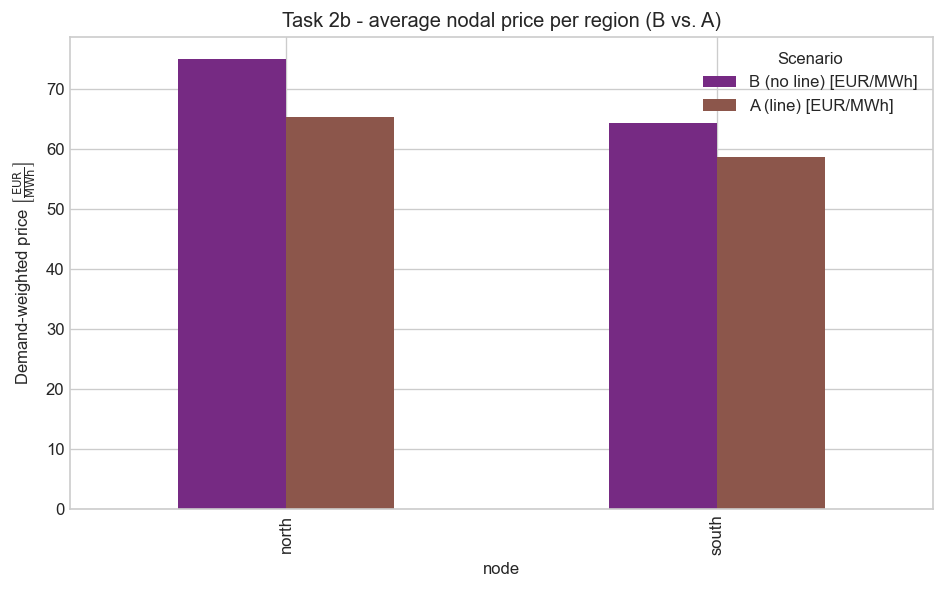
\includegraphics[width=0.75\linewidth]{Images/fig_2b_prices.png}
    \caption{Demand-weighted average nodal price per region in scenarios A (line) and B (no line).}
    \label{fig:2b_prices}
\end{figure}


\textbf{
    (c) Extract the shadow price of the line capacity constraint in the transmission scenario. What does it represent? In the scenario where the transmission capacity is zero, you can also extract the dual variable. Comparing the two, what does it say about the value of interconnection? (0.5)
    }

The shadow price of the line capacity constraint is obtained by summing the duals of the upper and lower transmission flow constraints over all time steps.
\autoref{fig:2c_line} illustrates the comparison between the two scenarios.

\begin{figure}[!htbp]
    \centering
    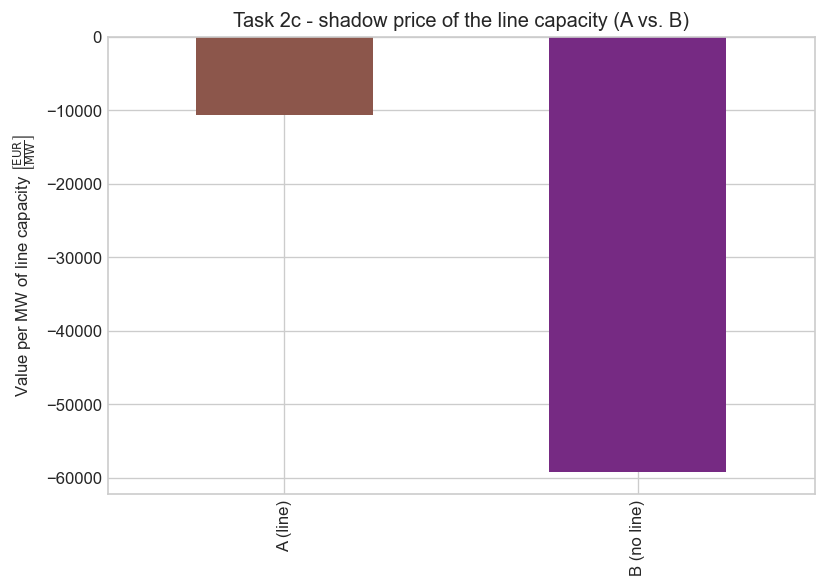
\includegraphics[width=0.65\linewidth]{Images/fig_2c_line.png}
    \caption{Shadow price of the line capacity constraint in scenarios A (line) and B (no line).}
    \label{fig:2c_line}
\end{figure}

The shadow price represents the congestion rent: how much the total system cost would drop if the line could carry one more MW.
It corresponds to the price difference between north and south in the hours when the line is operating at its capacity limit. \\
In scenario A (line), the shadow price is small (about $-11\,\frac{\text{kEUR}}{\text{MW}}$).
Since the model is free to optimise the line capacity, it expands the line until the marginal benefit of one additional MW equals its annualised investment cost, so the residual marginal value is close to zero by construction. \\
In scenario B (no line), the line capacity is forced to zero.
The no-line constraint reflects the value of the very first MW of interconnection (about $-59\,\frac{\text{kEUR}}{\text{MW}}$).
This value is roughly $5.6$ times larger than the marginal value in scenario A, illustrating strongly decreasing returns to interconnection.
Interconnection is highly valuable, but with clearly decreasing value.
The first connections yield the greatest cost savings and additional capacity is built only as long as its marginal benefit exceeds its marginal cost.

\textbf{
    (d) Which advantages and disadvantages of heavy reliance on cross-regional interconnection does this stylised model not capture? No calculation needed. (0.5)
    }

The model captures the cost minimising value of interconnection under idealised conditions, but neglects several important real world effects. \\
Disadvantages not captured: \\
Highly interconnected systems are susceptible to cascade failures and systemic risk not representable in a lossless single-line model. Cross-border operation requires regulatory coordination and is exposed to political risk such as unilateral export restrictions. Large transmission projects also face public acceptance barriers that can delay or prevent construction. \\
Advantages not captured: \\
Beyond direct cost savings, interconnection improves system security by enabling imports during local shortfalls, reduces local market power, and promotes price convergence. The two-node topology also ignores meshed grid benefits such as N-1 security and reactive power support, so the model understates the true social value of interconnection.
Overall, the model provides a partial view of the true social value of interconnection, since it omits both the non-market benefits and the systemic risks that become relevant at high integration levels.